
\documentclass[10pt]{article}
\usepackage[utf8]{inputenc}
\usepackage{graphicx}
\usepackage{amsmath, amssymb}
\usepackage{geometry}
\usepackage{caption} 
\geometry{a4paper, margin=0.5in, landscape} 

\begin{document}

\section*{Comparative EIS Kinetics Report}
\textbf{Model Structure:} \texttt{R0-p(R1,CPE1)} \\
\textbf{Used data:} altered data, first 9 points removed and points with $freq > 2e+04$ removed

\begin{center}
    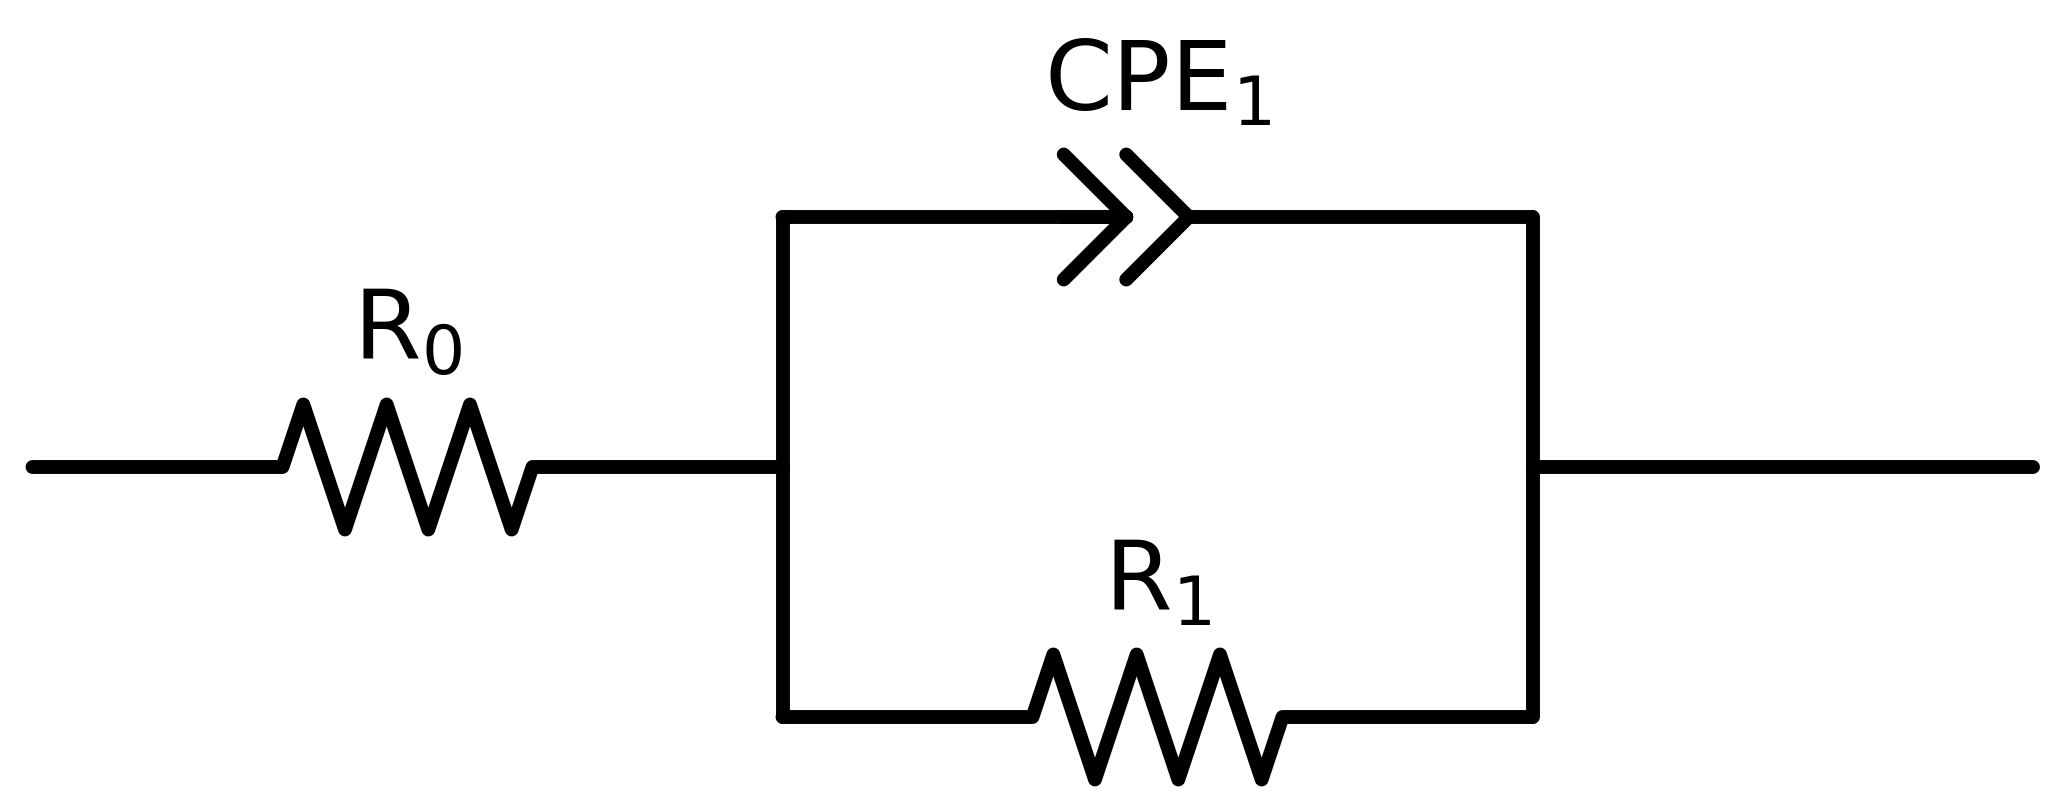
\includegraphics[width=0.45\textwidth]{../../1RC.png}
\end{center}

\renewcommand{\arraystretch}{1.6} 
\begin{table}[h!]
    \centering
    \footnotesize
    \begin{tabular}{|l|c|c|c|}
        \hline
        \textbf{Element} & \textbf{Unit} & \textbf{Bounds} & \textbf{Cauvel\_3\_BTA\_1H} \\ \hline
        $R_{0}$ & $\Omega$ & $[1.0e-03, 1.0e+03]$ & $7.76e+01 \pm 1.2e+00$ \\ \hline
        $R_{1}$ & $\Omega$ & $[1.0e+00, 1.0e+08]$ & $7.33e+04 \pm 2.3e+03$ \\ \hline
        $Q_{1}$ & $\Omega$$^{-1}$ sec$^{a}$ & $[1.0e-11, 1.0e-03]$ & $1.00e-05 \pm 2.1e-07$ \\ \hline
        $n_{1}$ & - & $[5.0e-01, 1.0e+00]$ & $9.11e-01 \pm 4.3e-03$ \\ \hline
        \textbf{$\chi^2$} & - & -  & $3.506e-03$ \\ \hline

    \end{tabular}
\end{table}


\newpage
\section*{Analysis Results: 1H}
\begin{center}
    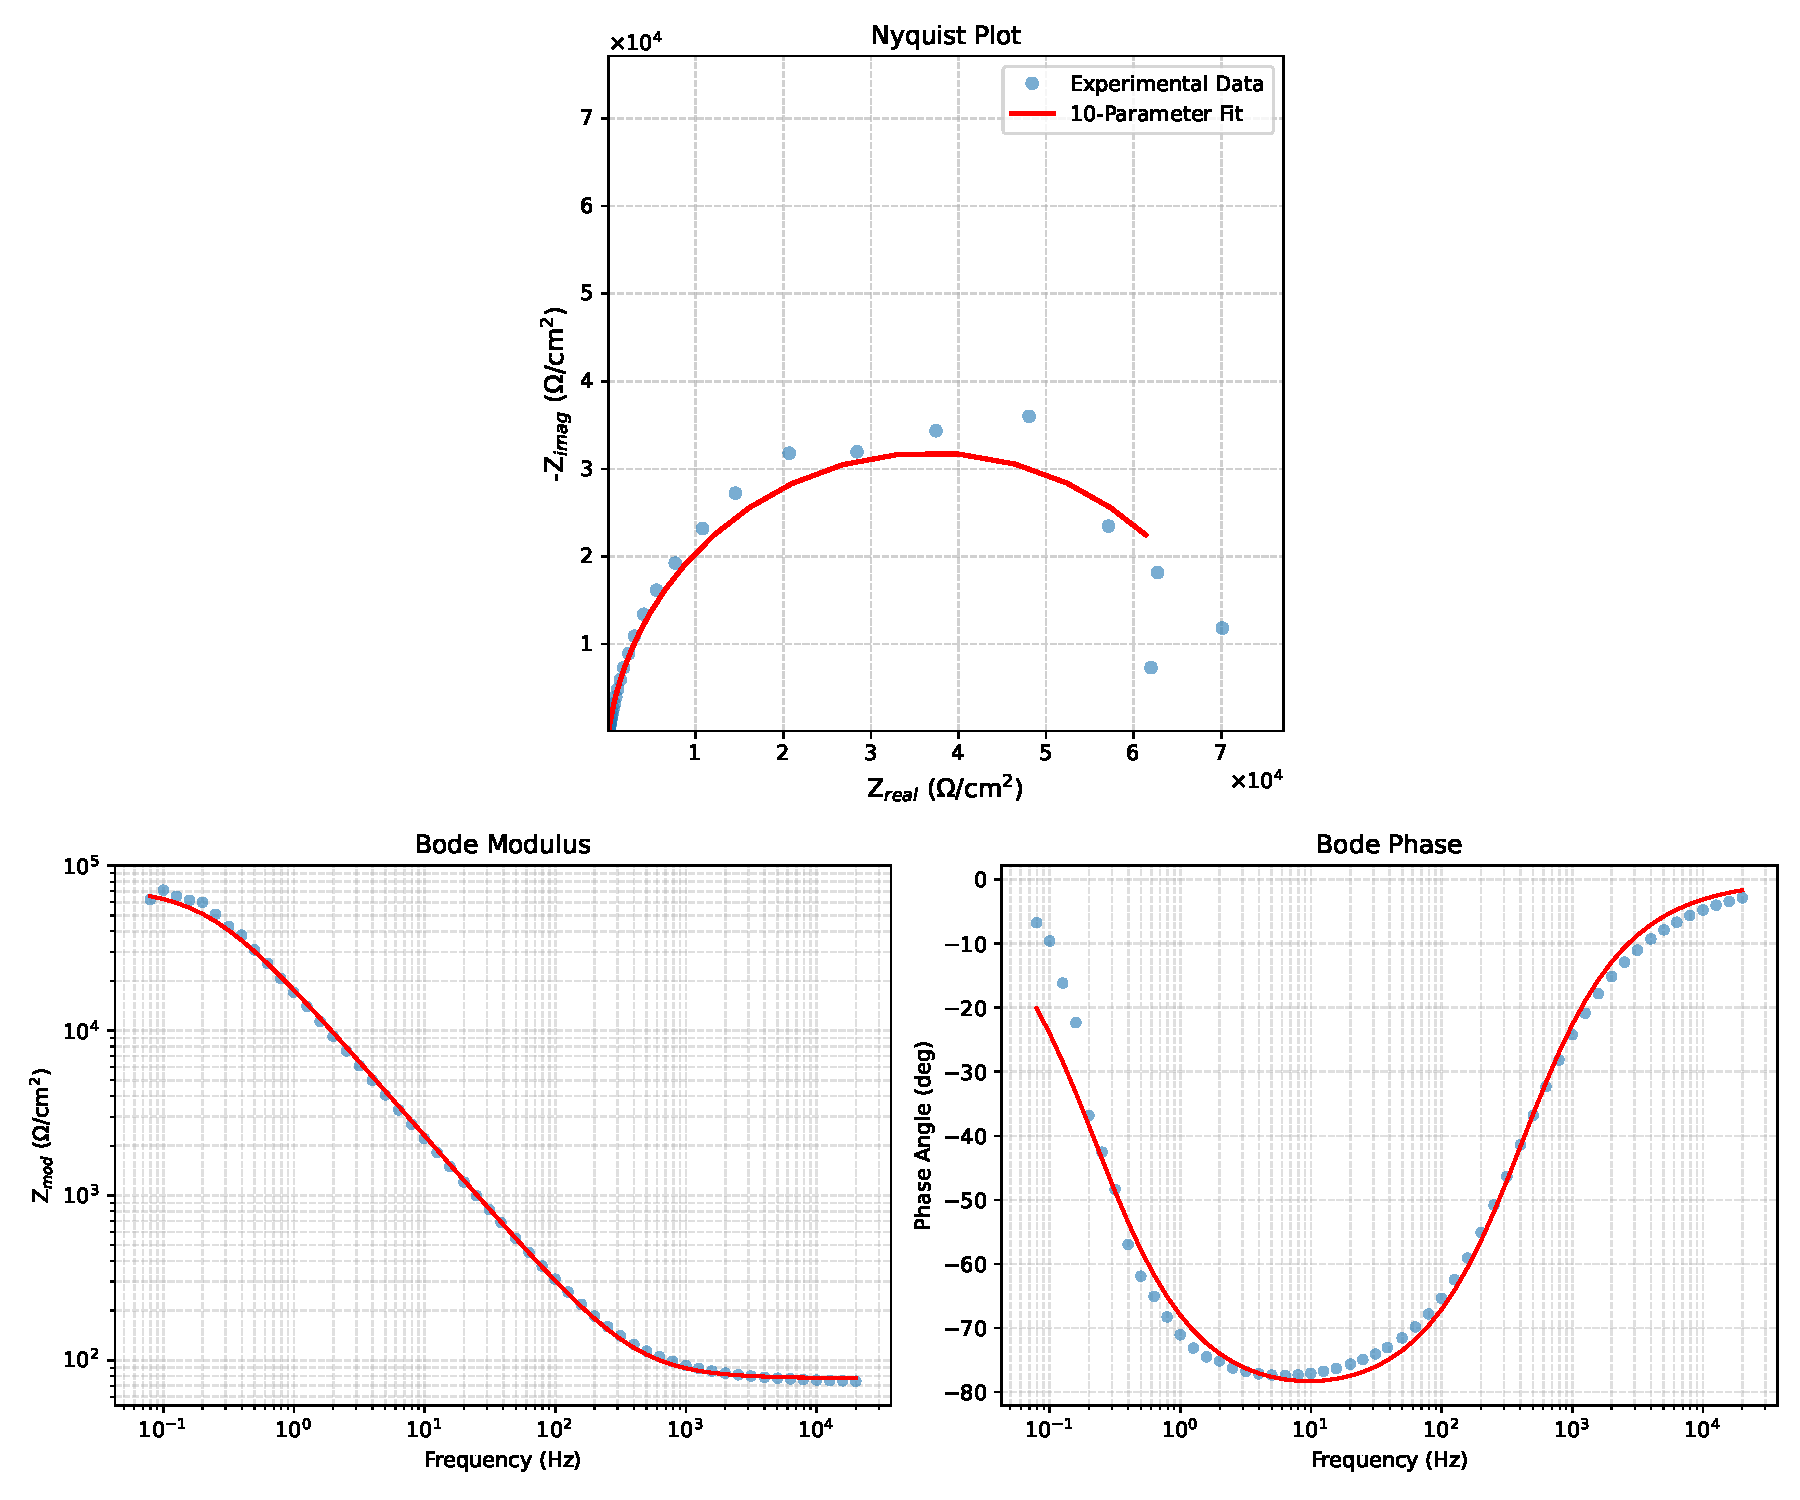
\includegraphics[width=0.7\textwidth]{plots_Cauvel_3_BTA_1H_1RC.pdf}
    \captionof{figure}{EIS Fit Results for Cauvel\_3\_BTA\_1H}
\end{center}


\end{document}
